\documentclass[a4paper,11pt]{article}

% Packages
\usepackage[T1]{fontenc}
\usepackage[fontsize=11pt]{scrextend}
\usepackage[margin=2cm, bottom=2cm,right=2cm]{geometry}
\usepackage{amsmath}
\usepackage{amssymb}
\usepackage{parskip}
\usepackage{tabularx}
\usepackage{float}
\usepackage{booktabs}
\usepackage{mathtools}
\usepackage{latexsym}
\usepackage{enumitem}
\usepackage{lastpage}
\usepackage{multicol}
\usepackage{listings}
\usepackage{pdflscape}

% Use Helvetica font (comment out to default to Computer Modern)
\usepackage{helvet}
\renewcommand\familydefault{\sfdefault}
\allowdisplaybreaks

% Tikz
\usepackage{tikz}
\usetikzlibrary{arrows,shapes,calc,math,decorations.fractals,patterns,backgrounds,decorations.markings}
\tikzset{bluevec/.style={-triangle 45,blue,line width=1pt}}
\tikzset{convex/.style={draw,ellipse}}
\tikzset{point/.style={fill,circle,inner sep=1.5pt}}

% Title
\title{Binary Space Partitioning}
\author{Dr Jon Shiach}
\date{March 2023}

\begin{document}

\maketitle

\subsection*{Example 36} 

The plan view of a world space is shown in the diagram below. The polygons labelled $A$ to $T$ to have norm vectors pointing into the interior. Construct a BSP tree for this world space.

\begin{center}
    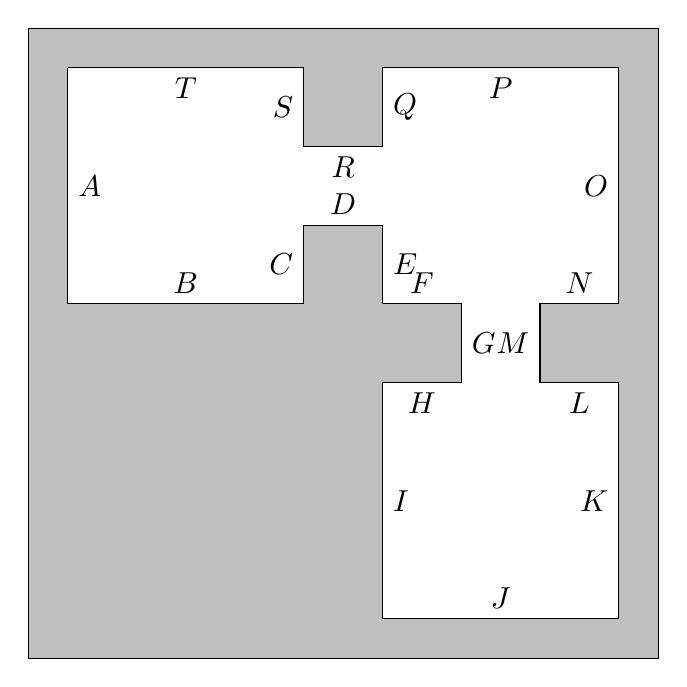
\begin{tikzpicture}[auto]
        \draw [fill=gray!50] (0,0) rectangle ++(8,-8);
        \draw [fill=white]
            (0.5,-0.5) -- node {$A$} ++(0,-3)
            -- node {$B$} ++(3,0)
            -- node {$C$} ++(0,1)
            -- node {$D$} ++(1,0)
            -- node {$E$} ++(0,-1)
            -- node {$F$} ++(1,0)
            -- node {$G$} ++(0,-1)
            -- node {$H$} ++(-1,0)
            -- node {$I$} ++(0,-3)
            -- node {$J$} ++(3,0)
            -- node {$K$} ++(0,3)
            -- node {$L$} ++(-1,0)
            -- node {$M$} ++(0,1)
            -- node {$N$} ++(1,0)
            -- node {$O$} ++(0,3)
            -- node {$P$} ++(-3,0)
            -- node {$Q$} ++(0,-1)
            -- node {$R$} ++(-1,0)
            -- node {$S$} ++(0,1)
            -- node {$T$} ++(-3,0);
    \end{tikzpicture}
\end{center}

\subsection*{Example 37}
Using the BSP given below, determine the rendering order for visible surface detection if the viewer is at position.

\begin{center}
    \resizebox{\textwidth}{!}{
        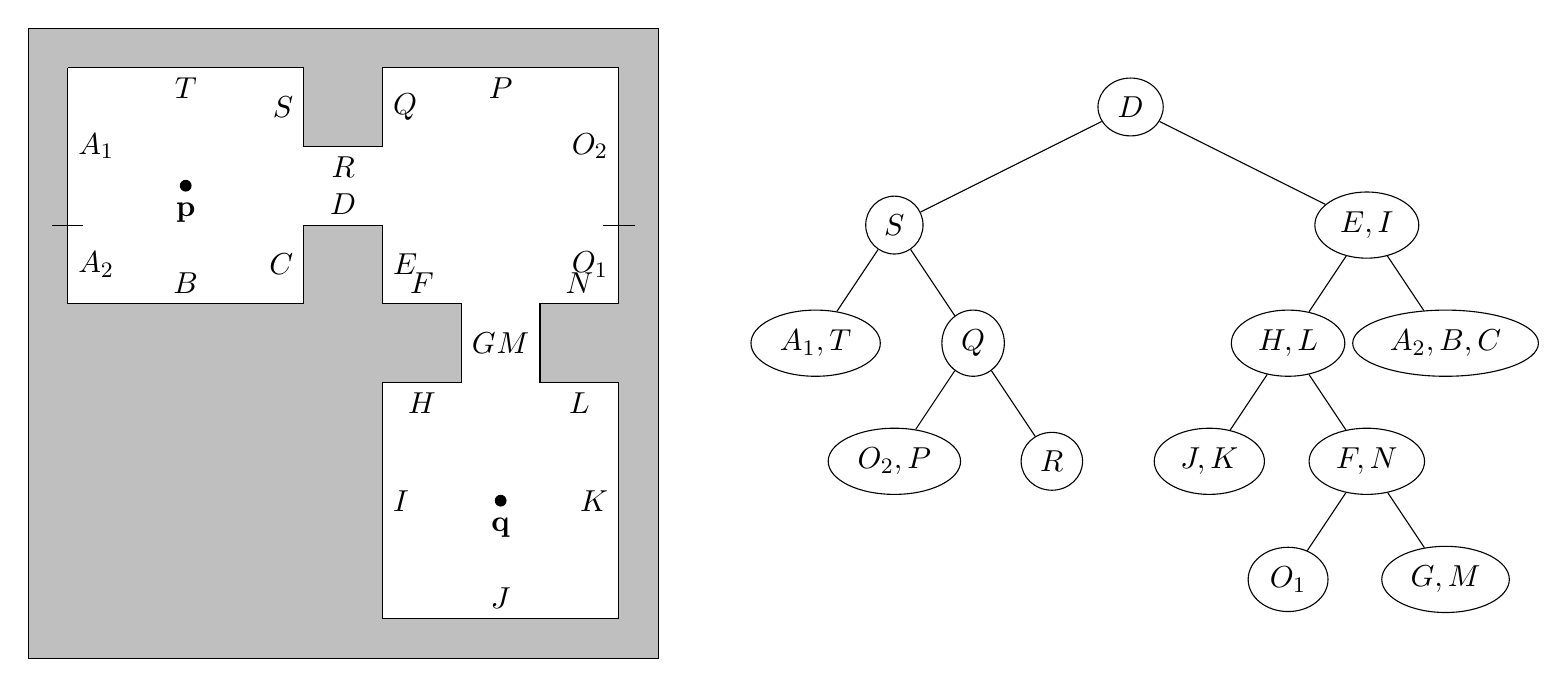
\begin{tikzpicture}[auto,
        level 1/.style={sibling distance=6cm},
        level 2/.style={sibling distance=2cm},
        level 3/.style={sibling distance=2cm}]
        \draw [fill=gray!50] (0,0) rectangle ++(8,-8);
        \draw [fill=white]
            (0.5,-0.5) -- node {$A_1$} ++(0,-2)
            -- node {$A_2$} ++(0,-1)
            -- node {$B$} ++(3,0)
            -- node {$C$} ++(0,1)
            -- node {$D$} ++(1,0)
            -- node {$E$} ++(0,-1)
            -- node {$F$} ++(1,0)
            -- node {$G$} ++(0,-1)
            -- node {$H$} ++(-1,0)
            -- node {$I$} ++(0,-3)
            -- node {$J$} ++(3,0)
            -- node {$K$} ++(0,3)
            -- node {$L$} ++(-1,0)
            -- node {$M$} ++(0,1)
            -- node {$N$} ++(1,0)
            -- node {$O_1$} ++(0,1)
            -- node {$O_2$} ++(0,2)
            -- node {$P$} ++(-3,0)
            -- node {$Q$} ++(0,-1)
            -- node {$R$} ++(-1,0)
            -- node {$S$} ++(0,1)
            -- node {$T$} ++(-3,0);
        \draw (0.3,-2.5) -- ++(0.4,0);
        \draw (7.3,-2.5) -- ++(0.4,0);
        \node at (14,-1) [convex] {$D$}
            child {node [convex] {$S$}
                child {node [convex] {$A_1, T$}}
                child {node [convex] {$Q$}
                    child {node [convex] {$O_2,P$}}
                    child {node [convex] {$R$}}
                }
            }
            child {node [convex] {$E,I$}
                child {node [convex] {$H,L$}
                    child {node [convex] {$J,K$}}
                    child {node [convex] {$F,N$}
                        child {node [convex] {$O_1$}}
                        child {node [convex] {$G,M$}}
                    }
                }
                child {node [convex] {$A_2, B, C$}}
            };
        \node [point,label=below:$\mathbf{p}$] at (2,-2) {};
        \node [point,label=below:$\mathbf{q}$] at (6,-6) {};
    \end{tikzpicture}
    }
\end{center}

\subsection*{Exercise 24}

A plan view of a map of a computer game is shown in the diagram below. Assuming all vectors are facing towards the interior, construct a BSP tree of the map.

\begin{center}
    \resizebox{0.8\textwidth}{!}{
    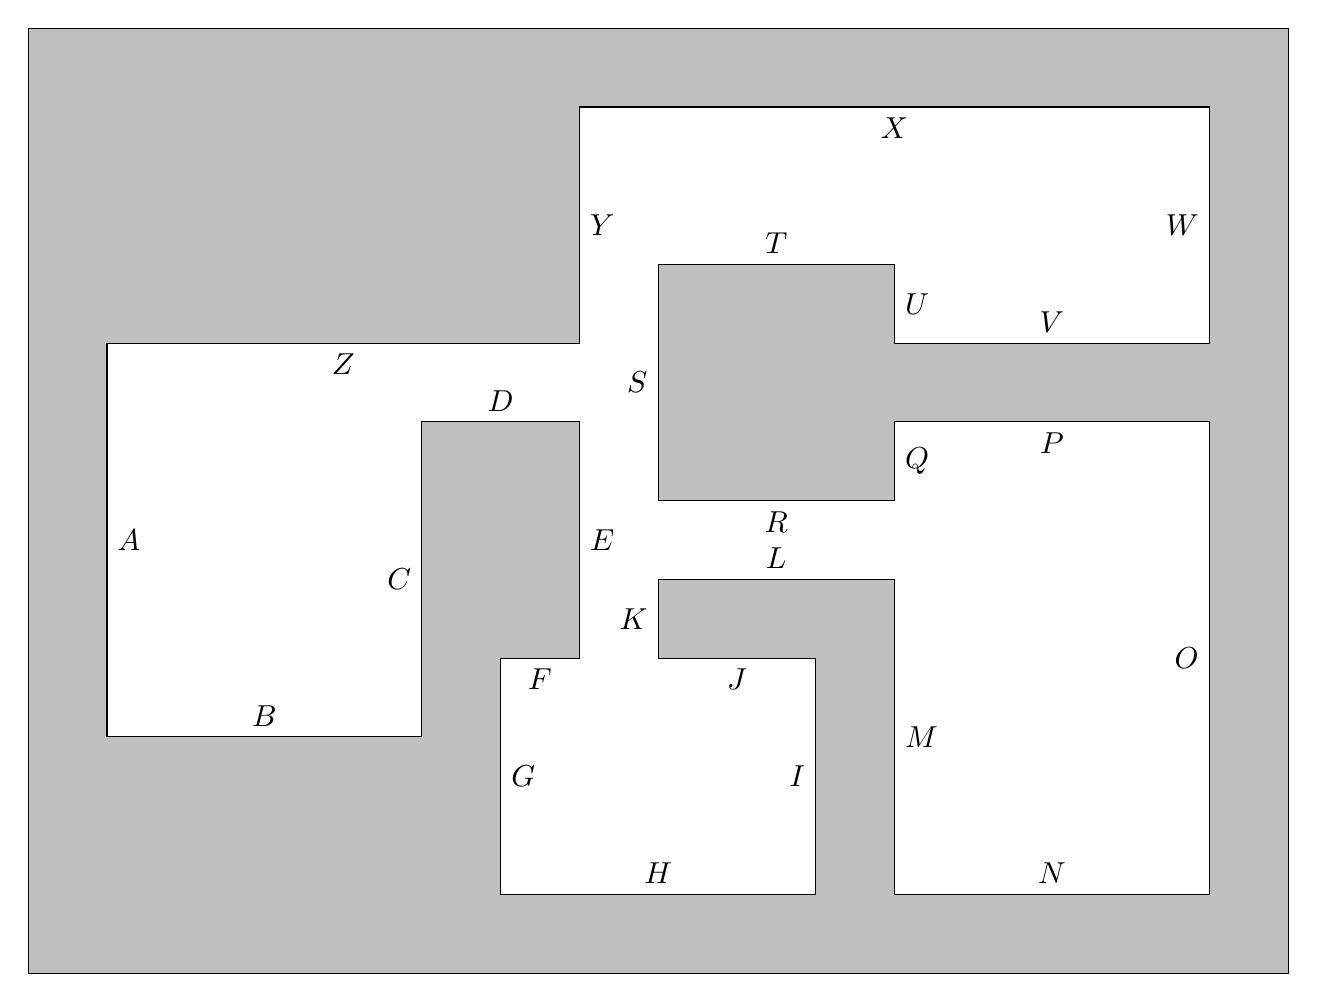
\begin{tikzpicture}[auto]
        \draw [fill=gray!50] (0,0) rectangle ++(16,-12);
        \draw [fill=white] (1,-4)
            -- node {$A$} ++(0,-5)
            -- node {$B$} ++(4,0)
            -- node {$C$} ++(0,4)
            -- node {$D$} ++(2,0)
            -- node {$E$} ++(0,-3)
            -- node {$F$} ++(-1,0)
            -- node {$G$} ++(0,-3)
            -- node {$H$} ++(4,0)
            -- node {$I$} ++(0,3)
            -- node {$J$} ++(-2,0)
            -- node {$K$} ++(0,1)
            -- node {$L$} ++(3,0)
            -- node {$M$} ++(0,-4)
            -- node {$N$} ++(4,0)
            -- node {$O$} ++(0,6)
            -- node {$P$} ++(-4,0)
            -- node {$Q$} ++(0,-1)
            -- node {$R$} ++(-3,0)
            -- node {$S$} ++(0,3)
            -- node {$T$} ++(3,0)
            -- node {$U$} ++(0,-1)
            -- node {$V$} ++(4,0)
            -- node {$W$} ++(0,3) 
            -- node {$X$} ++(-8,0)
            -- node {$Y$} ++(0,-3)
            -- node {$Z$} ++(-6,0);
    \end{tikzpicture}
    }
\end{center}

\subsection*{Exercise 25} 

A solution to Exercise 24 is shown below. Determine the rendering order of the polygons when the world is viewed from the positions $\mathbf{p}$, $\mathbf{q}$ and $\mathbf{r}$.

\begin{center}
    \resizebox{\textwidth}{!}{
    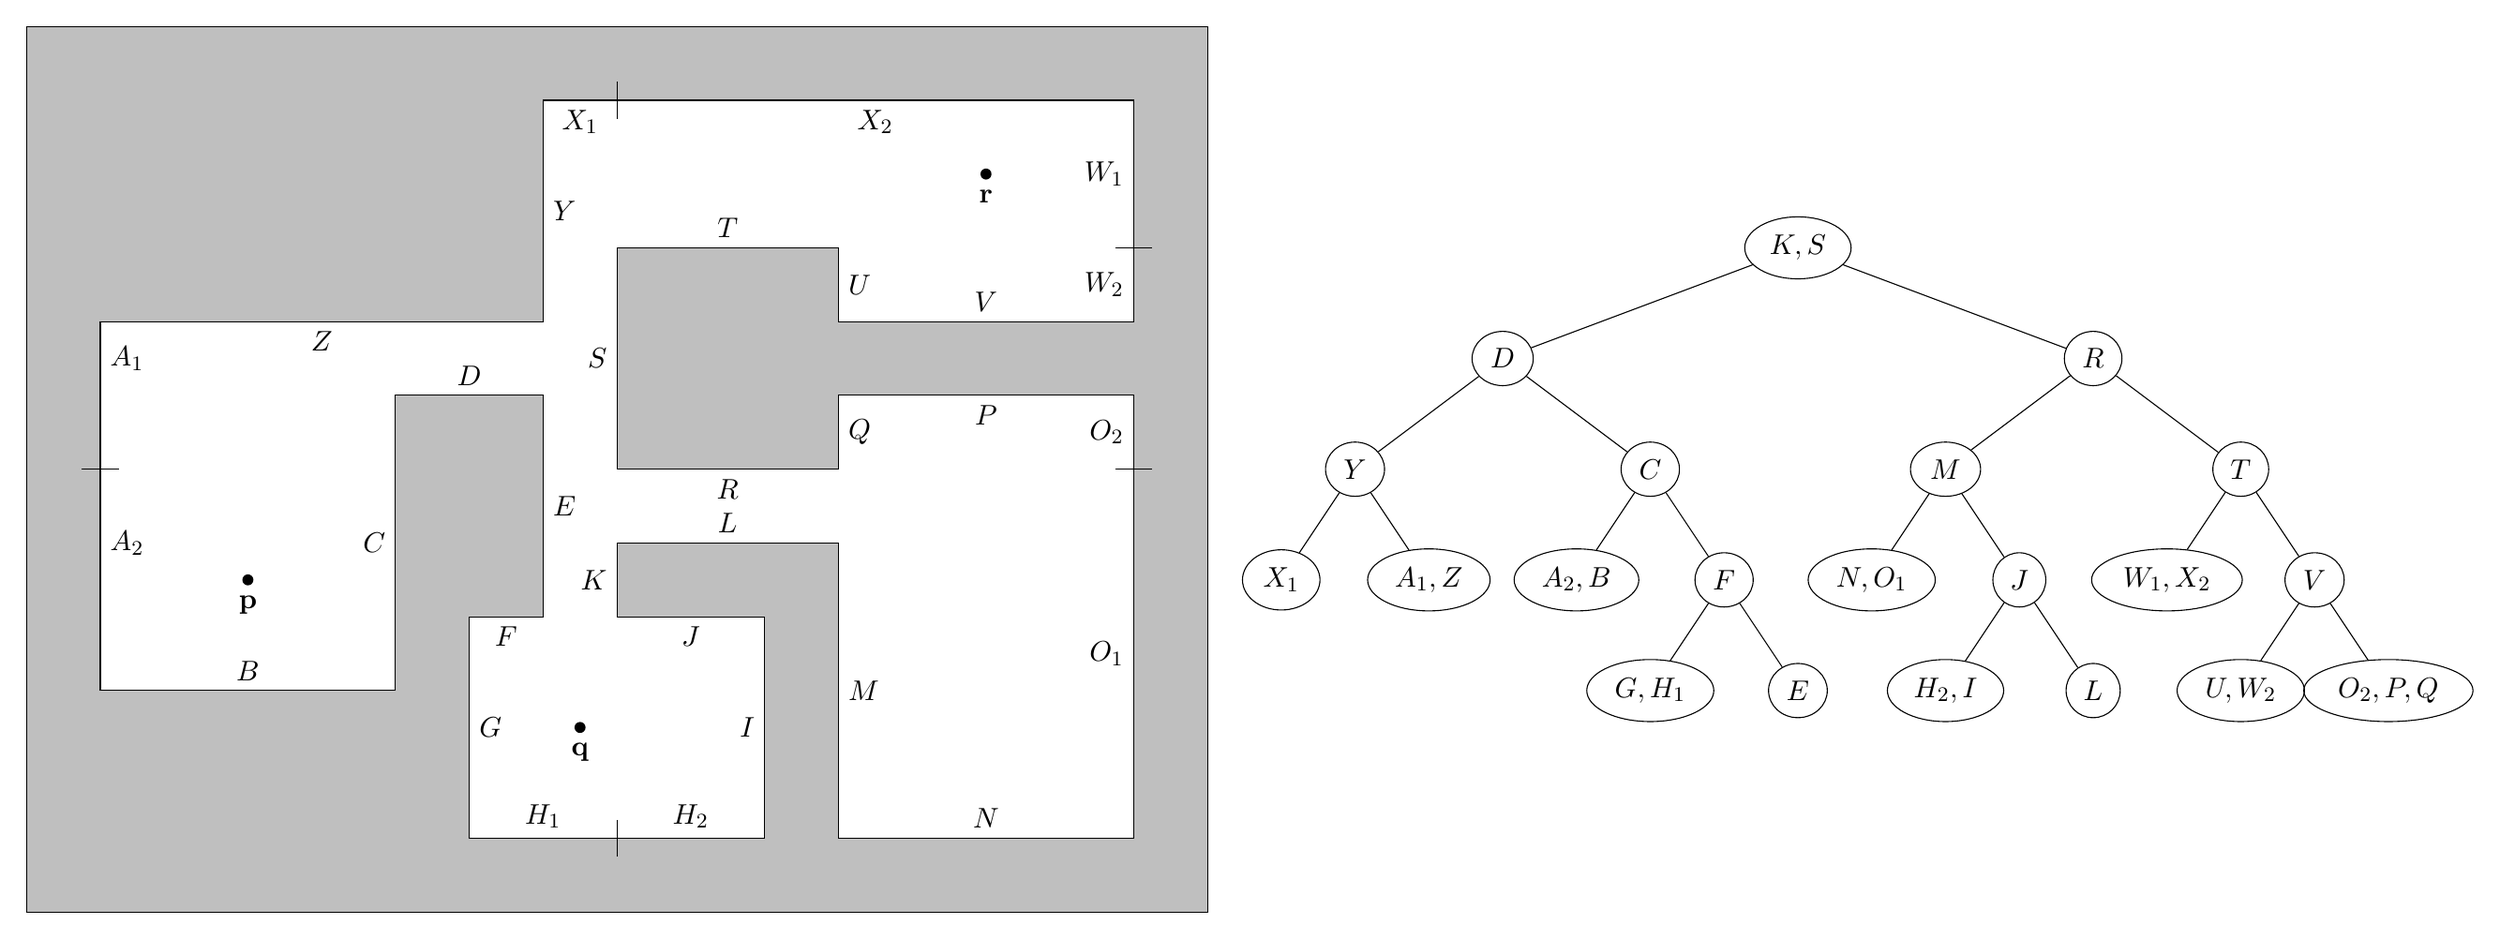
\begin{tikzpicture}[auto,
        level 1/.style={sibling distance=8cm},
        level 2/.style={sibling distance=4cm},
        level 3/.style={sibling distance=2cm},
        level 4/.style={sibling distance=2cm},
    ]
        \draw [fill=gray!50] (0,0) rectangle ++(16,-12);
        \draw [fill=white] (1,-4)
            -- node {$A_1$} ++(0,-1)
            -- node {$A_2$} ++(0,-4)
            -- node {$B$} ++(4,0)
            -- node {$C$} ++(0,4)
            -- node {$D$} ++(2,0)
            -- node {$E$} ++(0,-3)
            -- node {$F$} ++(-1,0)
            -- node {$G$} ++(0,-3)
            -- node {$H_1$} ++(2,0)
            -- node {$H_2$} ++(2,0)
            -- node {$I$} ++(0,3)
            -- node {$J$} ++(-2,0)
            -- node {$K$} ++(0,1)
            -- node {$L$} ++(3,0)
            -- node {$M$} ++(0,-4)
            -- node {$N$} ++(4,0)
            -- node {$O_1$} ++(0,5)
            -- node {$O_2$} ++(0,1)
            -- node {$P$} ++(-4,0)
            -- node {$Q$} ++(0,-1)
            -- node {$R$} ++(-3,0)
            -- node {$S$} ++(0,3)
            -- node {$T$} ++(3,0)
            -- node {$U$} ++(0,-1)
            -- node {$V$} ++(4,0)
            -- node {$W_2$} ++(0,1)
            -- node {$W_1$} ++(0,2) 
            -- node {$X_2$} ++(-7,0)
            -- node {$X_1$} ++(-1,0)
            -- node {$Y$} ++(0,-3)
            -- node {$Z$} ++(-6,0);
        \node [point,label=below:$\mathbf{p}$] at (3, -7.5) {};
        \node [point,label=below:$\mathbf{q}$] at (7.5, -9.5) {};
        \node [point,label=below:$\mathbf{r}$] at (13, -2) {};
        \draw (0.75,-6) -- ++(0.5,0);
        \draw (8,-11.25) -- ++(0,0.5);
        \draw (14.75,-6) -- ++(0.5,0);
        \draw (14.75,-3) -- ++(0.5,0);
        \draw (8,-1.25) -- ++(0,0.5);
    \node [convex] at (24, -3) {$K,S$}
        child { node [convex] {$D$} 
            child { node [convex] {$Y$} 
                child { node [convex] {$X_1$} }
                child { node [convex] {$A_1, Z$} }
            }
            child { node [convex] {$C$}
                child { node [convex] {$A_2, B$} }
                child { node [convex] {$F$}
                    child { node [convex] {$G, H_1$} }
                    child { node [convex] {$E$} }
                }
            }
        }
        child { node [convex] {$R$} 
            child { node [convex] {$M$} 
                child { node [convex] {$N, O_1$} }
                child { node [convex] {$J$} 
                    child { node [convex] {$H_2,I$} }
                    child { node [convex] {$L$} }
                }
            }
            child { node [convex] {$T$} 
                child { node [convex] {$W_1, X_2$} }
                child { node [convex] {$V$} 
                    child { node [convex] {$U,W_2$} }
                    child { node [convex] {$O_2,P,Q$} }
                }
            }
        };
    \end{tikzpicture}
    }
\end{center}

\end{document}